\section{Andre patterns}
Ved sammeligning af \textbf{CQRS} og andre patterns er det nærliggende at inddrage \textbf{CRUD}.

Begge disse patterns bruges til, at tilgå og skrive data på en Database, men deres metoder er forskellige. Forskellen udspiller sig i måden de er implementeret på og derfor også måden de operere på.\newline

På understående figur \ref{fig:CRUDimpl} nedenfor kan det ses, hvordan \textbf{CRUD}-implementeringen ved hjælp af sin \textit{Data-access}-klasse både tilgår og skriver data på databasen. Derimod er dette separeret på figur \ref{fig:CQRSimpl} dette fremgår også af figur \ref{fig:class-one} og \ref{fig:class-two}

\begin{figure}[H]
	\centering
	\begin{minipage}{.5\textwidth}
		\centering
		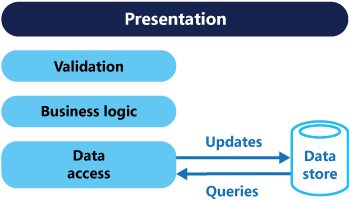
\includegraphics[width=.6\linewidth]{CRUDImplementation.png}
		\captionof{figure}{\textbf{CRUD}-Implemantation \cite{MicrosoftCQRS}}
		\label{fig:CRUDimpl}
	\end{minipage}%
	\begin{minipage}{.5\textwidth}
		\centering
		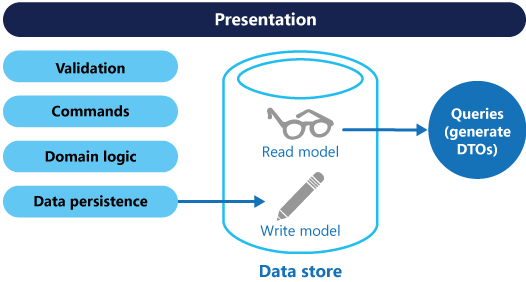
\includegraphics[width=.7\linewidth]{CQRSImplementation}
		\captionof{figure}{\textbf{CQRS}-Implemtation \cite{MicrosoftCQRS}}
		\label{fig:CQRSimpl}
	\end{minipage}
\end{figure}


Ved at separere læse og skrive operationerne opnås skaleringsmuligheder der med \textbf{CRUD} ikke er mulige. Grunden til dette er individualiseringen af både læse og skriver klasser, samt de afhængigheder de ikke deler.\newline

Derudover behøver disse ikke at udvikles 1:1.\newline

Den største forskel på de to patterns udspiller sig i, at \textbf{CRUD} udvikles som regel med \textbf{DDD} \textbf{D}omain \textbf{D}riven \textbf{D}esign, hvorimod \textbf{CQRS} udvikles ofte i et begivenhedsdrevet design (Event Driven Design). som navnene antyder bliver det domæne drevne design bygget op af domæner som figurer i den virkelige verden, hvorimod eventdriven design er bygget op om begivenheder der sker. som f.eks. at en kunde bestiller en kop kaffe.

Ved til dels at opbygget et system om det eventdrevne princip og at adskille læse/skrive-operationer mødes nogle problematikker som skal løses. Disse problemer gør, at \textbf{CQRS} kun bruges når systemet opnår en vis størrelse og kompleksitet, men at \textbf{CQRS} forstrækkes når dette niveau opnås.\newline

Ved implementering af \textbf{CQRS} gøres der brug af eventsourcing, som også vil blive omtalt herefter. I korte træk er det den del der sørger for, at fuldende den eventdrevne tankegang og underbygge reaktion indbyrdes i pattern'et.
Det er dog nævneværdigt, at eventsourcing ikke er en del af selve \textbf{CQRS}-pattern'et men at det ofte bliver implementeret ved brug af \textbf{CQRS}, da man på den måde løser nogle af ovenstående problemer.

